\subsection{Circle Packing}
\label{sec:circle-packing}


Circle packing considers arrangements of circles on surfaces
with the property that no two circles overlap. 
Dense packings are often desirable \cite{chang_simple_2010}.
In dense circle packings, all circles are touching other circles.
Given a circle packing one can construct the \emph{contact graph} with a vertex for each
circle and an edge connecting tangent circles.

A disk triangulation graph is a graph $G=(V,E)$ that is planar, all interior faces
are triangles, the boundary of $G$ forms a simple closed polygonal chain, and each
vertex has finite degree (locally finite).  See \figref{circle-packing} for an example.
In \todo{find citation} proved the following remarkable theorem.

\begin{theorem}[Koebe-Andreev-Thurston (KAT)]\label{thm:kat}
Every finite, simple, planar graph can be represented as a circle packing in the plane.
\end{theorem}

\begin{figure}[htb]
        \centering
        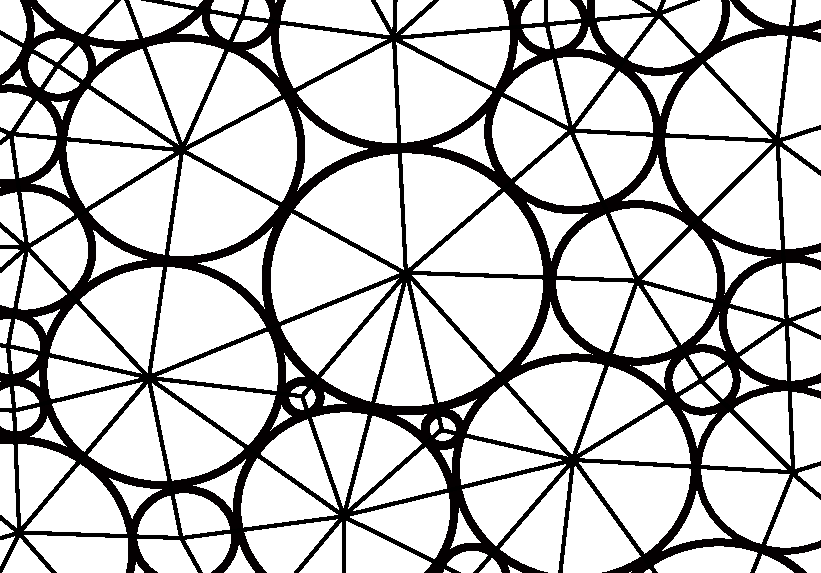
\includegraphics[width=.45\textwidth]{circle-packing}
		\caption{Part of an infinite circle packing and its corresponding contact graph.
		\label{fig:circle-packing}}
\end{figure}


Given disk triangulation graph, the corresponding circle packing guaranteed
by \thmref{kat} assigns angles around all vertices in $V$.
Thus, for each vertex we can compute its discrete curvature given by
the circle packing,
$$K(v)=2\pi -\sum_{\text{angles at } v}\theta_i,$$
assigns a value to each vertex.
The Gauss-Bonnet theorem holds using this circle packing metric on the vertices
of graphs which are used to model many important relationships.


Not all infinite planar graphs are flat, some may be negatively curved \cite{higuchi_combinatorial_2001}.
The combinatorial curvature at $v$ is
\begin{equation}\label{eqn:combinatorial-curvature}
\kappa(v)=1-\frac{\deg v}{2}+\sum_{f\sim v}\frac{1}{\deg f}
\end{equation}
where $\deg f $ is the number of edges in a face (three in a triangulation graph) and
the summation is over all faces incident to $v.$ 
If we associate each face $f$ with a regular $(\deg f)$-gon
of side length one, and glue the faces along sides determined by $G$, then 
we obtain a polygonal surface and 
\eqnref{combinatorial-curvature} agrees with our notion of curvature defined earlier only
scaled so that $2\pi$ becomes one.

If our graph has a boundary we have a notion of geodesic curvature.
Let $\Gamma=[v_0,v_1,\ldots, v_{n-1},v_n=v_0]$ be a cycle of length $n\geq 3.$
For each $k=1,2,\ldots, n$ let $f_1^k,f_2^k,\ldots f_{s_k}^k$ be the faces incident to $v_k$
lying on the right of the path $[v_{k-1},v_k,v_{k+1}],$ then the \emph{outer left turn} at $v_k$
is defined to be
\begin{equation}\label{eqn:outer-left}
\tau_o(v_k)=\sum_{j=1}^{s_k}\left(\frac{1}{2}-\frac{1}{\deg f_j^k}\right)-\frac{1}{2},
\end{equation}
and the outer left turn of the boundary $\Gamma$ is $\tau_o(\Gamma)=\sum_{k=1}^n\tau_o(v_k)$.

For a subgraph $S$ of $G$ a disk triangulation graph, we have the following formulation of the Gauss-Bonnet theorem. Define $dS$ as the vertex boundary of $S$, the set of vertices with neighbors both in and not in $S$. Also define $\partial S$ to be the edge boundary of $S$, the set of edges incident to a vertex in $S$ and a vertex not in $S$. Finally, define $bS$ to be the union of the boundary walks of $S$, $bS$ is the union of cycles determined by walking along the boundary of $D(S)=S\cup \left(\cup_{f\in F(S)}f\right).$


\begin{theorem}[Circle Packing Gauss-Bonnet]\label{thm:CPGB}
If $G$ is an infinite disk triangulation graph and $S\subset G$ a connected finite subgraph of $G.$
Then 
$$\kappa(S)+\tau_o(bS)=\chi(S),$$
where $\kappa(S)=\sum_{v\in V(S)}\kappa (v).$
\end{theorem}

\begin{proof}
	For a small $\epsilon>0,$ let $P$ be the polygonal region in $S_G$ obtained
	from a $\epsilon$-neighborhood of $D(S)$ with sharp corners.
	Let $bP$ be the topological boundary of $P$ and $\tau(bP)$ be the total left turn, or the 
	geodesic curvature, of $bP.$ Then, one can check that 
	$$\tau(bP)=2\pi \tau_o(bS).$$
	The polyhedral surface $S_G$ is locally Euclidean except the vertices of $G$.
	Then $\kappa(\text{int} (P))=2\pi \kappa(S)$ and the theorem follows from the Gauss-Bonnet Theorem
	for polyhedral surfaces.
\end{proof}

\todo{gauss-bonnet all up in here\cite{gu_discrete_2013}}


Given an infinite disk triangulation graph $G$ with no information about
its circle packing, the corresponding circle packing either fills
the entire plane or it fills the unit disk.
The plane and the disk cannot be mapped bijectively to each other, thus
we can define the circle packing type. A disk triangulation graph $G$ is circle packing
 \emph{parabolic} if there exits a circle packing which fill the entire plane 
 whose contact graph is equivalent to $G,$ and $G$ is circle packing \emph{hyperbolic}
 if there exists a circle packing which fill the unit disk and whose contact graph
 is equivalent to $G$.

Suppose we are presented with a graph $G$ of disk triangulation with an infinite 
number of vertices, our task is to determine if $G$ is parabolic or hyperbolic
We next share an application of the Gauss-Bonnet theorem given by Oh in \cite{oh_criteria_2022},
to make this determination.


Other criteria for determining the circle packing type of a disk triangulation graph exist.
A graph is \emph{recurrent} if a simple random walk returns to the start with probability one
and is \emph{transient} if there is a non-zero probability that a random walk does not return.
In \cite{he_hyperbolic_1995}, He and Schramm showed that if $G$ is recurrent, then $G$
is parabolic and if $G$ is transient and of bounded degree then $G$ is hyperbolic.

In general they showed that a if $G$ has a `large' number of vertices with 'large' degree
then $G$ is parabolic. More specifically
\begin{itemize}
\item if at at most finitely vertices in $G$ have degrees greater than six, then $G$ is parabolic.
\item if the inequality holds
\begin{equation}\label{eqn:He-Sch-hyper}
\sup_{S_0}\inf_{S_0\subset S}\left(\frac{1}{|S_0|}\sum_{v\in S}\deg v \right)>6
\end{equation}
where $S_0$ and $S$ are nonempty connected finite subgraphs of $G$, then
$G$ is hyperbolic.
\end{itemize}
The inequality in \eqnref{He-Sch-hyper} can be thought of as the average degree 
in a `region' of $G$ being greater than six.
Repp proved the following stronger result \cite{repp_bounded_2001}.
If the sequence
\begin{equation}\label{eqn:repp}
k_n=\sum_{v\in B_n}(\deg v - 6)
\end{equation}
is bounded, where $B_n$ is the combinatorial ball of radius $n$ (meaning the number of edges
between a vertex and the center vertex is at most $n$) and centered at a fixed vertex,
then $G$ is parabolic.
This sequence $k_n$ is the \emph{degree excess} sequence.
The Gauss-Bonnet theorem to improve the gap between the above
statement in the following way.

\begin{theorem}\label{thm:Oh-packing}
For each $n\in\NN$ let $B_n$ be the combinatorial ball of radius $n$
centered at a fixed vertex in $G.$ Let $k_n$ be the degree excess sequence
defined above, let $a_n=\sum_{j=0}^{n-1}(k_j+6)$ for $n=1,2,\ldots$.
Then $G$ is circle-packing parabolic if 

\begin{equation}\label{eqn:cp-parabolic}
\sum_{n=1}^{\infty}\frac{1}{a_n}=\infty,
\end{equation}

and $G$ is recurrent if

\begin{equation}\label{eqn:recurrent}
\sum_{n=1}^{\infty}\frac{1}{a_n+a_{n+1}}=\infty.
\end{equation}

\end{theorem}

As a consequence we have if

$$k_n=\sum_{v\in B_n}(\deg v -6)\leq c\ln n$$
for sufficiently large $n$, where $c$ is a fixed positive constant,
then $G$ is circle-packing parabolic and recurrent.

Before providing details we sketch the general idea of the proof of \thmref{Oh-packing}.
For the ball $B_n$ we consider the curvature $\kappa(B_n),$ 
and check that it is a constant multiple of the degree excess sequence $k_n.$
By considering the geodesic curvature on the boundary of $B_n,$ 
a formula involving the number of edges connecting edges of $B_n$
to the rest of the graph.
The Gauss-Bonnet theorem relates the degree excess sequence to
the number of boundary edges. For a combinatorial sphere
$S_n$ of radius $n$ centered at a fixed vertex, and $E_n$ is the set of edges
connecting $B_n$ to the rest of the graph, and show
$$|S_n|\leq \sum_{j=0}^{n-1}(k_j+6)=a_n \text{ and } |E_n|\leq a_n + a_{n+1},$$


